\chapter{基本概念与相关工作}\label{chap:Relate}

本章节主要介绍SMT和非线性实数理论的相关基本概念以及研究现状。首先,本文给出SMT问题和非线性实数理论的语法,然后给出解空间表达以帮助读者更好地理解SMT问题的本质。紧接着本文给出CDCL(T)算法的结构、MCSAT算法原理以及其他一些SMT求解器的介绍。然后给出近几年来局部搜索在SMT问题上的应用,包括线性整数逻辑、多线性逻辑和部分多项式理论等。最后,本文总结目前算法的缺点和非线性问题的挑战,并引出本工作带来的进展和突破。

\section{可满足性模理论与非线性实数问题}
首先,本文给出可满足行模理论(Satisfiability Modulo Theories, SMT)问题的一般定义,前置概念介绍如下:

\begin{definition}{\textbf{变量 (Variable)}}
SMT问题中的变量根据赋值要求分为布尔变量和算术变量。布尔变量是只能取布尔值($\top, \bot$)的变量,布尔变量集合一般用$B$表示。算术变量可以取整数或者实数值,一般用$R$表示。非线性实数问题中所有算术变量必须取实数值。
\end{definition}

\begin{definition}{\textbf{多项式约束 (Polynomial Constraint)}}
非线性问题主要由多项式约束构成,多项式约束的形式为$P(x) \sim 0$,其中$P(x)$是一个多项式,$\sim$是一个关系符号,可以是$\{=, <, >\}$中的一个。比如,$x^2 + y > 0$是一个多项式约束。
\end{definition}

\begin{definition}{\textbf{线性约束 (Linear Constraint)}}
线性约束是每一项都是线性项(只有一个次数为1的变量)的多项式约束,形如$\sum_{i=1}^n a_i x_i \sim 0$,其中$a_i$是常数项,$x_i$是变量。比如,$x + y + z = 1$是一个线性约束。
\end{definition}

\begin{definition}{\textbf{多线性约束 (Multilinear Constraint)}}
多线性约束是一种特殊的多项式约束,其中多项式中的每一项的变量次数不能超过1次,即每一项的每一个变量次数都是1。比如,$x y + y z k < 0$是一个多线性约束。
\end{definition}

\begin{definition}{\textbf{Tseitin编码(Tseitin Encoding)}}
Tseitin编码具体做法是为每一个子公式引入一个新变量,然后写出新变量和原来子公式之间的等价关系,最后将所有的等价关系和原公式的子公式一起写成CNF形式。Tseitin编码的优点是可以有效地减少公式的大小,并且保持了公式的可满足性。
\end{definition}

鉴于Tseitin编码的能力,为方便说明,本文中所有SMT约束表达成为CNF形式,一些基本概念如下:
\begin{definition}{\textbf{命题文字 (Literal)}}
命题文字是可满足问题中的基本结构,包括正文字($p$)和负文字($\neg p$)。非线性实数理论的命题文字一般是多项式约束或布尔变量约束。正文字只有当对应的多项式约束满足时才满足,负文字只有当对应的多项式约束不满足时才满足。一个典型的非线性实数文字比如$x^2 + y > 0$或者$\neg (x + y^3 < 0)$。
\end{definition}

\begin{definition}{\textbf{子句 (Clause)}}
子句定义为文字的析取结构,一般记为$C = l_1 \vee l_2 \vee \dots \vee l_n$,其中$l_i$是一个文字。当子句包含的所有文字不满足时子句不满足,只要有一个文字被满足子句也被满足。\textbf{空子句 (empty clause)}一般表示不包含任何文字的子句。比如,一个非线性实数理论的子句形如$(x^2 + y > 0) \vee (x + y^3 < 0)$。
\end{definition}

\begin{definition}{\textbf{公式 (Formula)}}
公式定义为子句的合取结构,一般记为$\varphi = C_1 \wedge C_2 \wedge \dots \wedge C_m$,其中$C_i$是一个子句。当公式包含的所有子句都满足时公式满足,只要有一个子句不满足公式就不满足。一个非线性实数理论的公式比如$(x^2 + y > 0) \wedge (x + y^3 < 0)$。
\end{definition}

对于非线性实数理论来说,文字、子句和公式的关系可以由以下形式化定义:
\begin{align*}
\textbf{多项式:} \quad & p := x | c | p + p | p \cdot p \\
\textbf{文字:} \quad & l := b | p \leq 0 | p \geq 0 | p = 0 \\
\textbf{子句:} \quad & C := l_1 \vee l_2 \vee \dots \vee l_n \\
\textbf{公式:} \quad & \varphi := C_1 \wedge C_2 \wedge \dots \wedge C_m
\end{align*}
多项式可以是变量$x$,常数$c$,或者两个多项式的加和以及乘积构成;文字可以是单一的布尔变量$b$,多项式构成的不等式$p \leq 0$,$p \geq 0$或者$p = 0$;子句是多个文字的析取;公式是多个子句的合取。

\begin{definition}{\textbf{赋值 (Assignment)}}
赋值指的是变量到布尔值或者实数的一种映射,布尔变量赋值为$f: B \rightarrow \{\top, \bot\}$,算术变量赋值为$f: R \rightarrow \mathbb{R}$。一个赋值$f$满足一个公式$\varphi$,记作$f \models \varphi$,当且仅当对于公式中的每一个子句$C_i$,至少有一个文字$l_j$满足$f \models l_j$。赋值可以分为部分赋值(partial assignment)和完全赋值(full assignment),部分赋值只对部分变量存在映射,完全赋值对所有变量都存在映射。赋值一般记为一组映射,比如$\{x \mapsto 2, y \mapsto 3\}$。
\end{definition}

\begin{definition}{\textbf{评估 (Evaluation)}}
评估指的是给定赋值和一个文字,判断当前文字是否满足,记为$eval (ass, l) \rightarrow \{\top, \bot\}$,其中$ass$是一个赋值,$l$是一个文字。评估的结果为$\top$表示文字满足,为$\bot$表示文字不满足。比如$eval (\{x \mapsto 2, y \mapsto 3\}, x^2 + y > 0) \rightarrow \top$。评估只有在文字包含的所有变量都有赋值时才有返回值。
\end{definition}

\begin{definition}{\textbf{可满足性模理论(Satisfiability Modulo Theories, SMT)}}
可满足性模理论(SMT)指的是给定一个逻辑公式$\varphi$,如果存在一组赋值$f$使得$f \models \varphi$,则称$\varphi$是\textbf{可满足的(satisfiable)},否则称$\varphi$是\textbf{不可满足的(unsatisfiable)}。SMT问题的目标是找到一个可满足的赋值,即找到一个满足公式的赋值,或者证明赋值不可满足。
\end{definition}

例\ref{ex:SMT}进一步说明SMT问题的可满足性。

\begin{example}
\label{ex:SMT}
给定SMT公式$\varphi = (x^2 + y > 0) \wedge (x + y^3 < 0)$,可以找到一组赋值$f = \{x \mapsto 2, y \mapsto -2\}$使得$f \models \varphi$。因此称该问题是可满足的。给定SMT公式$\varphi = (x^2 + y^2 < 0)$,在实数空间上找不到一组赋值满足当前约束,因此该问题是不可满足的。
\end{example}


\textbf{逻辑公式化简:} 为方便说明,本文把所有的算术文字化简为以下几种形式$\{p > 0, p \geq 0, p = 0\}$,其中$p$是多项式。具体的化简规则表述如下:
\begin{itemize}
    \item $p < 0$化简为$p' > 0$,其中$p'$表示$p$的相反多项式。
    \item $p \leq 0$化简为$p' \geq 0$,其中$p'$表示$p$的相反多项式。
    \item $p \leq 0 \wedge p \geq 0$化简为$p = 0$。
\end{itemize}


\section{SMT(NRA)的解空间}
本小节主要探讨SMT(NRA)公式的解空间结构,以帮助读者更好理解SMT问题和搜索过程的本质。
\subsection{多项式约束的解空间}
\begin{definition}{\textbf{解空间 (Solution Space)}}
解空间指的是满足SMT公式的所有赋值的集合,一般用$S$表示。解空间是一个高维空间,每个维度对应一个变量的取值,每个点对应一个赋值。解空间的维度取决于变量的个数,解空间的大小取决于变量的取值范围。非线性实数的解空间是$R^n$,其中$n$是公式包含的变量个数。
\end{definition}
\begin{example}
    \begin{figure*}[]
        \centering
        \bicaption {解空间示意图} {Demo of Solution Space.}
        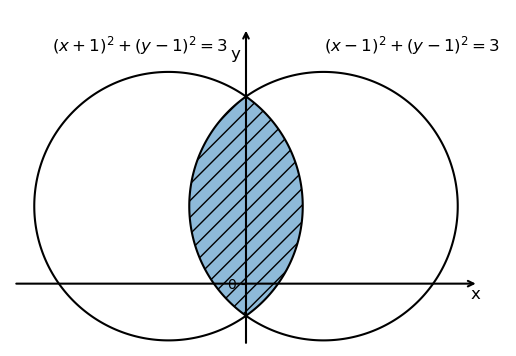
\includegraphics[width=0.4\columnwidth]{Img/cell1.png}
        \label{fig:solution_space}
    \end{figure*}
    
    考虑逻辑公式$F = (x - 1)^2 + (y - 1)^2 \le 3 \wedge (x + 1)^2 + (y - 1)^2 \le 3$,构成的$R^2$空间图形如图\ref{fig:solution_space}所示。两个子句分别表示两个圆的内部,逻辑公式$F$表示同时存在两个圆内部的区域,即图中阴影区域。任何存在于阴影区域内的点都满足逻辑公式$F$,任何满足逻辑公式$F$的点都存在于阴影区域内。因此,解空间$S$是阴影区域的集合。
\label{ex:solution_space}
\end{example}
    
数学上,把符号一致的连通区域定义为胞腔。具体定义如\ref{def:cell}所示:

\begin{definition}{\textbf{胞腔 (Cell)}}
对于$R^n$空间上的多项式集合$Q$,$Q$的一个胞腔(cell)是每个多项式$P \in Q$保持符号不变的$R^n$最大连通集合。对于任意的点$a \in R^n$,如果$a$在$Q$的胞腔内,则$a$满足$Q$中的所有多项式,记这个胞腔为$cell(Q, a)$。显然,胞腔是$R^n$空间的一个划分。
\label{def:cell}
\end{definition}

对于逻辑公式而言,因为胞腔内的任意一点对每个多项式$P \in Q$保持符号不变,因此SMT公式对应的所有文字仍然保持布尔值不变,不会对SMT公式整体的满足或不满足造成任何影响。当找到其中任意一个满足逻辑公式的胞腔时,可以判定原公式可满足;当所有胞腔都被证明不可满足时,可以判定原公式不可满足。

给定逻辑公式,如何快速剔除不满足的胞腔并找到可满足的胞腔非常重要,因此现有的研究工作很多聚焦在更好地胞腔划分上。一般的胞腔划分是根据多项式的根和判别式等来判断的,从一个点得到胞腔的划分称为延拓。

\begin{definition}{\textbf{延拓 (Expansion)}}
假定$R^n$上的多项式集合$Q$和点$a = (a_1, ..., a_n)$。给定一个变量$x_i (i = 1, 2,..., n)$,假定多项式$
q(a_1, ..., a_{i-1}, x_i, a_{i+1}, ..., a_n)$的实数根为$r_1 < r_2 < \cdots < r_s$。一个点$a$关于变量$x_i$在集合$Q$上的延拓定义为一个满足如下性质的点集$\Lambda \subseteq R^n$:
\begin{itemize}
    \item 点$a \in \Lambda$并且对于$1 \leq j \leq s$均存在点$(a_1, ..., a_{i-1}, r_j, a_{i+1}, ..., a_n) \in \Lambda$。
    \item 对于任意点$b = (b_1, ..., b_n) \in \Lambda$,对于$j \in \{1, ..., n\} \setminus \{i\}$,有$b_j = a_j$。
    \item 对于任意的区间$I \in \{(-\infty, r_1), (r_1, r_2), \cdots, (r_{s-1}, r_s), (r_s, +\infty)\}$,存在唯一的$b = (b_1, ..., b_n) \in \Lambda$满足$b_i \in I$。
\end{itemize}
\textbf{点集的延拓:} 对于点集$\{a^{(1)}, ..., a^{(m)}\} \subseteq R^n$,定义集合关于变量$x_i$在$Q$上的延拓是$\bigcup_{j=1}^m \Lambda_j$,其中$\Lambda_j$是$a^{(j)}$关于变量$x_i$的延拓。
\end{definition}

\begin{example}
\begin{figure*}[]
    \centering
    \bicaption {延拓点集示意图} {Expansion Demo.}
    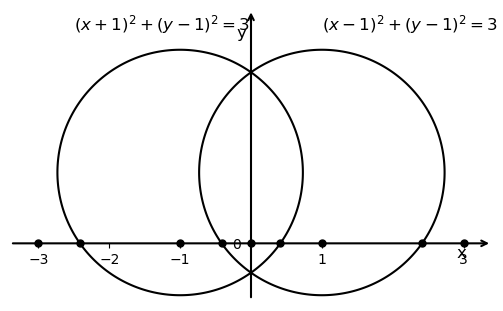
\includegraphics[width=0.45\columnwidth]{Img/cell2.png} \qquad
    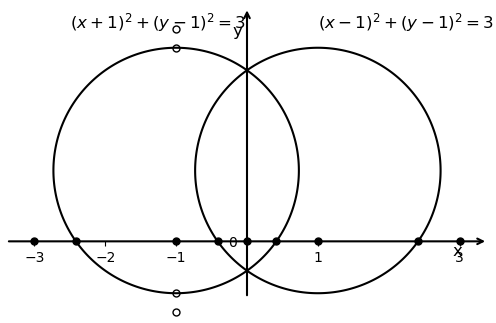
\includegraphics[width=0.45\columnwidth]{Img/cell3.png}
    \label{fig:expansion}
\end{figure*}
继续考虑例子\ref{ex:solution_space},如图\ref{fig:expansion}所示,可以得到点$(0, 0)$关于$x$的延拓,即点集$\{(-3, 0), (-1-\sqrt{2}, 0), (-1, 0), (1-\sqrt{2}, 0), (0, 0), (\sqrt{2} - 1, 0), (1, 0), (1+\sqrt{2}, 0), (3, 0)\}$。这些点在$x$变量上分割了多项式的符号区间,从而划分了胞腔在$x$方向上的投影。右侧图的空心点构成了点$(-1, 0)$关于变量$y$的延拓,即点集$\{(-1, -1), (-1, 1-\sqrt{3}), (-1, 1+\sqrt{3}), (-1, 3)\}$,这些点在$y$方向上分开了多项式的符号区间,从而划分了胞腔在$y$方向上的投影。
\label{ex:expansion1}
\end{example}
点$a$关于变量$x$的延拓点集事实上是点$a$在方向$x$上相邻胞腔的采样点,如何能够对$R^n$空间上的所有胞腔进行采样是本文接下来的话题。为此,引入柱形延拓的概念。

\begin{definition}{\textbf{柱形延拓 (Cylindrical Expansion)}}
假设$R^n$上的多项式集合$Q$和点$a$。给定一个变量顺序$x_1 < x_2 < \cdots < x_n$,定义点$a$关于变量顺序在$Q$上的柱形延拓是$\bigcup_{i=1}^n \Lambda_i$,其中$\Lambda_1$是$a$关于变量$x_1$在$Q$上的延拓,并且$\Lambda_{i+1}$是$\Lambda_i$关于变量$x_{i+1}$在$Q$上的延拓。把最终的结果$\bigcup_{i=1}^n \Lambda_i$称为$Q$上的柱形延拓。
\end{definition}

柱形延拓可以理解为给定变量顺序下多维的点集延拓,其目的是在$R^n$空间的每一个胞腔上都有一个采样点。
\begin{figure*}[]
    \centering
    \bicaption {柱形延拓示意图} {Cylindrical Expansion Demo.}
    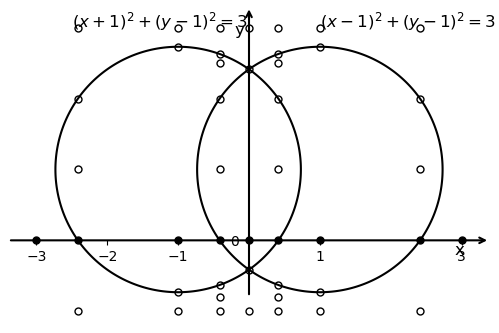
\includegraphics[width=0.5\columnwidth]{Img/cell4.png}
    \label{fig:expansion2}
\end{figure*}
\begin{example}

\begin{table*}[]
    % \tiny
    \centering
    \bicaption{柱形延拓-采样点生成} {Demo of Computation of Cylindrical Expansion-Sampling Points.}
    \resizebox{\linewidth}{!}{
        \begin{tabular}{c | c | c | c | c | c}
    \hline
    投影点1 & 分割区间1 & 延拓点集1(采样点1) & 投影点2 & 分割区间2 & 延拓点集2(采样点2)\\\hline
    
    (-3, 0) & $(-\infty, \infty)$ & (-3, 0) & (3, 0) & $(-\infty, \infty)$ & (3, 0) \\\hline
    
    \multirow{5}{*}{$(-1-\sqrt{2}, 0)$} & $(-\infty, 0)$ & $(-1-\sqrt{2}, -1)$ & \multirow{5}{*}{$(1+\sqrt{2}, 0)$} & $(-\infty, 0)$ & $(1+\sqrt{2}, -1)$ \\ & [0, 0] & $(-1-\sqrt{2}, 0)$ && [0, 0] & $(1 + \sqrt{2}, 0)$ \\ & (0, 2) & $(-1-\sqrt{2}, 1)$ && (0, 2) & $(1+\sqrt{2}, 1)$  \\ & [2, 2] & $(-1-\sqrt{2}, 2)$ && [2, 2] & $(1+\sqrt{2}, 2)$ \\ & $(2, \infty)$ & $(-1-\sqrt{2}, 3)$ && $(2, \infty)$ & $(1+\sqrt{2}, 3)$ \\\hline
    
    \multirow{5}{*}{(-1, 0)} & $(-\infty, 1-\sqrt{3})$ & (-1, -1) & \multirow{5}{*}{(1, 0)} & $(-\infty, 1-\sqrt{3})$ & (1, -1) \\
    & $[1-\sqrt{3}, 1-\sqrt{3}]$ & $(-1, 1-\sqrt{3})$ && $[1-\sqrt{3}, 1-\sqrt{3}]$ & $(1, 1-\sqrt{3})$ \\
    & $(1-\sqrt{3}, 1+\sqrt{3})$ & (-1, 0) && $(1-\sqrt{3}, 1+\sqrt{3})$ & $(1, 0)$ \\
    & $[1+\sqrt{3}, 1+\sqrt{3}]$ & $(-1, 1+\sqrt{3})$ && $[1+\sqrt{3}, 1+\sqrt{3}]$ & $(1, 1+\sqrt{3})$ \\
    & $(1+\sqrt{3}, \infty)$ & (-1, 3) && $(1+\sqrt{3}, \infty)$ & (1, 3) \\\hline 

    \multirow{9}{*}{$(1-\sqrt{2}, 0)$} & $(-\infty, -0.63)$ & $(1-\sqrt{2}, -1)$ & \multirow{9}{*}{$(1+\sqrt{2}, 0)$} & $(-\infty, -0.63)$ & $(1+\sqrt{2}, -1)$ \\
    & [-0.63, -0.63] & $(1-\sqrt{2}, -0.63)$ && [-0.63, -0.63] & $(1+\sqrt{2}, -0.63)$ \\
    & (-0.63, 0) & $(1-\sqrt{2}, -0.5)$ && (-0.63, 0) & $(\sqrt{2}-1, -0.5)$ \\
    & [0, 0] & $(1-\sqrt{2}, 0)$ && [0, 0] & $(\sqrt{2}-1, 0)$ \\
    & (0, 2) & $(1-\sqrt{2}, 1)$ && (0, 2) & $(\sqrt{2}-1, 1)$\\
    & [2, 2] & $(1-\sqrt{2}, 2)$ && [2, 2] & $(\sqrt{2}-1, 2)$ \\
    & (2, 2.63) & $(1-\sqrt{2}, 2.5)$ && (2, 2.63) & $(\sqrt{2}-1, 2.5)$  \\
    & [2.63, 2.63] & $(1-\sqrt{2}, 2.63)$ && [2.63, 2.63] & $(\sqrt{2}-1, 2.63)$\\
    & (2.63, \infty) & $(1-\sqrt{2}, 3)$ && $(2.63, \infty)$ & $(\sqrt{2}-1, 3)$ \\\hline

    \multirow{5}{*}{(0, 0)} & $(-\infty, 1-\sqrt{2})$ & $(0, -1)$ & \multirow{5}{*}{(0, 0)} & $(-\infty, 1-\sqrt{2})$ & $(0, -1)$ \\
    & $[1-\sqrt{2}, 1-\sqrt{2}]$ & $(0, 1-\sqrt{2})$ && $[1-\sqrt{2}, 1-\sqrt{2}]$ & $(0, 1-\sqrt{2})$ \\
    & $(1-\sqrt{2}, 1+\sqrt{2})$ & (0, 0)&& $(1-\sqrt{2}, 1+\sqrt{2})$ & (0, 0) \\
    & $[1+\sqrt{2}, 1+\sqrt{2}]$ & $(0, 1+\sqrt{2})$&& $[1+\sqrt{2}, 1+\sqrt{2}]$ & $(0, 1+\sqrt{2})$ \\
    & $(1+\sqrt{2}, \infty)$ & (0, 3)
    &&$(1+\sqrt{2}, \infty)$ & (0, 3)\\\hline
\end{tabular}
        }
\label{tab:expansion2}
\end{table*}

继续考虑例子\ref{ex:expansion1},如图\ref{fig:expansion2}所示,图中所有的实心点和空心点共同构成了基于变量顺序$x < y$的多项式$Q$的柱形延拓,达到了每个胞腔上均有一个采样点的效果。具体的步骤是,首先点$(0, 0)$关于变量$x$形成延拓(实心点),然后每一个实心点关于变量$y$各自形成延拓(空心点),最终所有点的集合共同构成了柱形延拓。表格\ref{tab:expansion}展示了在实心点处根据多项式集合的根分割得到的区间。表格\ref{tab:expansion2}展示了在每一个分割区间进行采样得到的结果,即最终的柱形延拓点集(空心点)。

\begin{table*}[]
    % \footnotesize
    \centering
    \bicaption{柱形延拓-区间计算} {Demo of Computation of Cylindrical Expansion-Interval Splitting.}
    % \setlength{\tabcolsep}{0.4mm}% column separation
    % \renewcommand{\arraystretch}{1.2}%row space 
    \resizebox{\linewidth}{!}{
        \begin{tabular}{c | c | c | c}
            \hline
            点坐标 & $P_1: (x+1)^2 + (y-1)^2 = 3$根 & $P_2: (x -1)^2 + (y-1)^2 = 3$根 & 根集合\\\hline
            $x \mapsto -3$ & \emptyset & \emptyset & \emptyset \\\hline
            $x \mapsto -1-\sqrt{2}$ & \{0, 2\} & \emptyset & \{0, 2\} \\\hline
            $x \mapsto -1$ & $\{1 - \sqrt{3}, 1 + \sqrt{3}\}$ & \emptyset & $\{1 - \sqrt{3}, 1 + \sqrt{3}\}$ \\\hline
            $x \mapsto 1-\sqrt{2}$ & \{-0.63, 2.63\} & \{0, 2\} & \{-0.63, 0, 2, 2.63\} \\\hline
            $x \mapsto 0$ & $\{1 - \sqrt{2}, 1 + \sqrt{2}\}$ & $\{1 - \sqrt{2}, 1 + \sqrt{2}\}$ & $\{1 - \sqrt{2}, 1 + \sqrt{2}\}$ \\\hline
            $x \mapsto \sqrt{2} - 1$ & \{0, 2\} & \{-0.63, 2.63\} & \{-0.63, 0, 2, 2.63\} \\\hline
            $x \mapsto 1$ & \emptyset & $\{1 - \sqrt{3}, 1 + \sqrt{3}\}$ & $\{1 - \sqrt{3}, 1 + \sqrt{3}\}$ \\\hline
            $x \mapsto 1+\sqrt{2}$ & \emptyset & \{0, 2\} & \{0, 2\} \\\hline
            $x \mapsto 3$ & \emptyset & \emptyset & \emptyset \\\hline
        \end{tabular}
        }
\label{tab:expansion}
\end{table*}
\end{example}

\begin{definition}{\textbf{柱形完备 (Cylindrical Complete)}}
对于$R^n$上的多项式集合$Q$,给定一个变量顺序$x_1 < x_2 < \cdots < x_n$,称$Q$对于变量顺序是柱形完备的,当任意的点$a \in R^n$和其关于$Q$的柱形延拓$\Lambda$,$Q$的每一个胞腔都包含至少一个$\Lambda$的点。具体的证明请参阅文献\cite{Caviness2004QuantifierEA,Collins74}。
\end{definition}

\subsection{量词消去与柱形代数分解}
根据前文的讨论,本文引出基于多项式解空间的一种量词消去算法-柱形代数分解(Cylindrical Algebraic Decomposition, CAD)。

\begin{definition}{\textbf{量词消去 (Quantifier Elimination)}}
量词消去指的是给定一个带有量词的逻辑公式$\varphi$,找到另一个不带有量词的逻辑公式$\psi$,使得$\varphi$和$\psi$的逻辑等价,记为$\varphi \Leftrightarrow \psi$。量词消去的目的是将逻辑公式转化为更易处理的形式,以更好地判断问题的可满足性。
\end{definition}

\begin{example}
考虑多项式$P_s(x, y) = s(x^2 + y^2 - 1) + (1 - s)(xy - 1)$,和逻辑公式$\varphi = \exists R \forall x, y [P_s(x, y) = 0 \Rightarrow x^2 + y^2 \leq R^2]$。量词消去即求解当$s$取什么值的时候逻辑公式$\varphi$满足。通过量词消去工具,本文可以得到$\varphi \Leftrightarrow s \le -1 \wedge s > \frac{1}{3}$。\label{ex:quantifier_elimination}
\end{example}

多项式理论常用的一种量词消去是柱形代数分解(Cylindrical Algebraic Decomposition, CAD)。其核心仍然是把$R^n$空间划分成多个符号一致的胞腔,然后通过判断每个胞腔是否满足逻辑公式进而得到给定变量的赋值区间。给定变量顺序和多项式集合,柱形代数分解可以分为三个步骤:投影、实根隔离和提升,具体的步骤如下:
\begin{itemize}
    \item \textbf{投影(projection):}从多项式集合开始,每次消去一个变量,生成新的多项式集合,新多项式继续消去变量直到只剩下一个变量为止,记为$proj(P)$。
    \item \textbf{实根隔离(root isolation):}当投影只剩下一个变量时,对当前多项式集合求所有根,得到顺序排列的一组根,这些根把$R$划分成了不同区间,对应胞腔在该方向上分割。
    \item \textbf{提升(lift):}提升是对投影阶段得到的多项式集合进行采样。投影从单变量多项式开始,从采样点继续对上一个投影多项式进行采样,直到最终对$R^n$多项式采样,最终保证了每个胞腔得到了采样点。
\end{itemize}

投影算子(projection operator)指的是投影过程中对多项式集合的计算,比如Collins算子\cite{Collins74}和McCallum算子\cite{McCallum98}。后者因为其计算相对便捷,被广泛应用于量词消去工具和SMT求解器中。为方便说明投影算子的计算,本文先简要介绍以下几种多项式操作:

\begin{definition}{\textbf{结式(Resultant)}}
对于两个多项式$P_1, P_2 \in R[x_1, ..., x_n]$,假定$$
P_1 = a_m x_n^{d_m} + a_{m-1} x_n^{d_{m-1}} + \cdots + a_0,
$$
$$
P_2 = b_n x_n^{e_n} + b_{n-1} x_n^{e_{n-1}} + \cdots + b_0.
$$
定义$P_1$和$P_2$的结式$Res(P_1, P_2, x_n)$为:
$$
Res(P_1, P_2, x_n) = 
\begin{vmatrix}
    a_m & a_{m-1} & \cdots & a_0 \\
    & a_m & a_{m-1} & \cdots & a_0 \\
    & \ddots & \ddots & \ddots & \ddots & \\
    & & a_m & a_{m-1} & \cdots & a_0 \\

    b_n & b_{n-1} & \cdots & b_0 \\
    & b_n & b_{n-1} & \cdots & b_0 \\
    & \ddots & \ddots & \ddots & \ddots & \\
    & & b_n & b_{n-1} & \cdots & b_0 \\
    \end{vmatrix}
$$
\end{definition}

\begin{definition}{\textbf{判别式(Discreminant)}}

对于多项式$P \in R[x_1, ..., x_n]$,假定$$
P = a_m x_n^{d_m} + a_{m-1} x_n^{d_{m-1}} + \cdots + a_0.
$$
定义$P$关于变量$x_n$的判别式$Disc(P, x_n)$为:  
$$
Disc(P, x_n) = \frac{(-1)^{\frac{m(m-1)}{2}}}{a_m} Res(f, \frac{\partial f}{\partial x_n}, x_n). 
$$
\end{definition}

\begin{definition}{\textbf{McCallum算子(McCallum Operator)}}
    假设当前多项式集合为$F = \{P_1, P_2, \dots, P_m\} \in R^n$,投影变量为$x_i$,McCallum算子$proj(F, x_i)$是从$F$到$R^{n-1}$上的多项式集合$proj_m(F)$的一组映射,包含以下元素:
    \begin{itemize}
        \item $F$中每个多项式的系数,记为$coeff(P_i)$
        \item $F$中每个多项式关于变量$x_i$的判别式,记为$disc(P_i, x_i)$
        \item $F$中每两个不同多项式$P_i, P_j$关于变量$x_i$的结式,记为$res(P_i, P_j, x_i)$
    \end{itemize}
    最终得到的多项式集合是三次计算得到的集合的并集,即$proj_m(F) = (\bigcup_{j=1 \cdots m} coeff(P_j)) \cup (\bigcup_{j=1 \cdots m} disc(P_j, x_i)) \cup (\bigcup_{j=1 \cdots m, k \neq j} res(P_j, P_k, x_i))$。
\end{definition}

\begin{example}
\begin{figure*}[t]
    \centering
    \bicaption {柱形代数分解步骤示意图} {Demo of Cylindrical Algebraic Decomposition Steps.}
    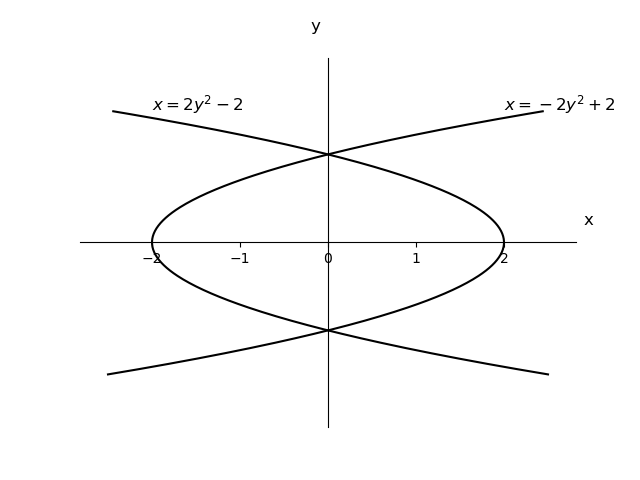
\includegraphics[width=0.6\columnwidth]{Img/cad.png}
\label{fig:CAD}
\end{figure*}

下面给出CAD算法的一个例子,如图\ref{fig:CAD}所示。假设$F = \{P_1: x - 2y^2 + 2, P_2: x + 2y^2 - 2\}$,规定变量顺序为$y < x$,按步骤计算如下:
\begin{enumerate}
    \item \textbf{投影}:计算对于变量$y$的投影$proj(F, y)$
    \begin{itemize}
        \item 化简后系数多项式集合为$\{x + 2, x - 2\}$
        \item 化简后判别式集合为$\{x + 2, x - 2\}$
        \item 化简后结式集合为$\{x\}$。
    \end{itemize}
    取并集得到投影多项式集合$proj(F, y) = \{x, x - 2, x + 2\}$

    \item \textbf{实根隔离}:对$proj(F, y)$的每个多项式求根,得到根集合$\{-2, 0, 2\}$。
    \item \textbf{提升}:对根集合分得的区间进行提升,进一步采样所有胞腔,结果如表格\ref{tab:cad}所示(忽略边界处的胞腔)。
    \begin{table*}
        % \tiny
        \centering
        \bicaption{柱形代数分解-提升} {Demo of Cylindrical Algebraic Decomposition - Lift.}
        \resizebox{\linewidth}{!}{
            \begin{tabular}{c | c | c}
            \hline
            胞腔符号 & 对应区间 & 采样点坐标 \\\hline
            $C_1$ & $x < -2 \wedge y > \sqrt{\frac{2 - x}{2}}$& (-2.4, 1.7) \\\hline
            $C_2$ & $x < -2 \wedge -\sqrt{\frac{2 - x}{2}} < y < \sqrt{\frac{2 - x}{2}} $ &(-2.4, 0) \\\hline
            $C_3$ & $x < -2 \wedge y < -\sqrt{\frac{x - 2}{2}}$ & (-2.4, -1.7) \\\hline

            $C_4$ & $-2 < x < 0 \wedge y > \sqrt{\frac{2 - x}{2}}$ & (-1, 1.7) \\\hline
            $C_5$ & $-2 < x < 0 \wedge \sqrt{\frac{2 + x}{2}} < y < \sqrt{\frac{2 - x}{2}}$ & (-1, 1)\\\hline
            $C_6$ & $-2 < x < 0 \wedge -\sqrt{\frac{2 + x}{2}} < y < \sqrt{\frac{2 + x}{2}}$ & (-1, 0) \\\hline
            $C_7$ & $-2 < x < 0 \wedge -\sqrt{\frac{2 - x}{2}}< y < -\sqrt{\frac{2 + x}{2}}$ & (-1, -1) \\\hline
            $C_8$ & $-2 < x < 0 \wedge y < -\sqrt{\frac{2 - x}{2}}$ & (-1, -1.7) \\\hline

            $C_9$ & $0 < x < 2 \wedge y > \sqrt{\frac{2 + x}{2}}$ & (1, 1.7) \\\hline
            $C_{10}$ & $0 < x < 2 \wedge \sqrt{\frac{2 - x}{2}} < y < \sqrt{\frac{2 + x}{2}}$ & (1, 1) \\\hline
            $C_{11}$ & $0 < x < 2 \wedge -\sqrt{\frac{2 - x}{2}} < y < \sqrt{\frac{2 - x}{2}}$ & (1, 0) \\\hline
            $C_{12}$ & $0 < x < 2 \wedge -\sqrt{\frac{2 + x}{2}} < y < -\sqrt{\frac{2 - x}{2}}$ & (1, -1) \\\hline
            $C_{13}$ & $0 < x < 2 \wedge y < -\sqrt{\frac{2 + x}{2}}$ & (1, -1.7) \\\hline

            $C_{14}$ & $x > 2 \wedge y > \sqrt{\frac{2 + x}{2}}$ & (2.4, 1.7) \\\hline
            $C_{15}$ & $x > 2 \wedge \sqrt{\frac{2 + x}{2}} < y < \sqrt{\frac{2 + x}{2}}$ & (2.4, 0) \\\hline
            $C_{16}$ & $x > 2 \wedge y < -\sqrt{\frac{2 + x}{2}}$ & (2.4, -1.7) \\\hline
            \end{tabular}
        }
        \label{tab:cad}
    \end{table*}
\end{enumerate}
\label{ex:cad}    
\end{example}


\section{非线性实数理论求解现状}
整体来说,SAT和SMT问题的求解方法包括完备方法、局部搜索算法和混合求解方法。本文工作LS\_NRA属于局部搜索算法在非线性实数理论上的拓展。

% \begin{figure*}[t]
%     \centering
%     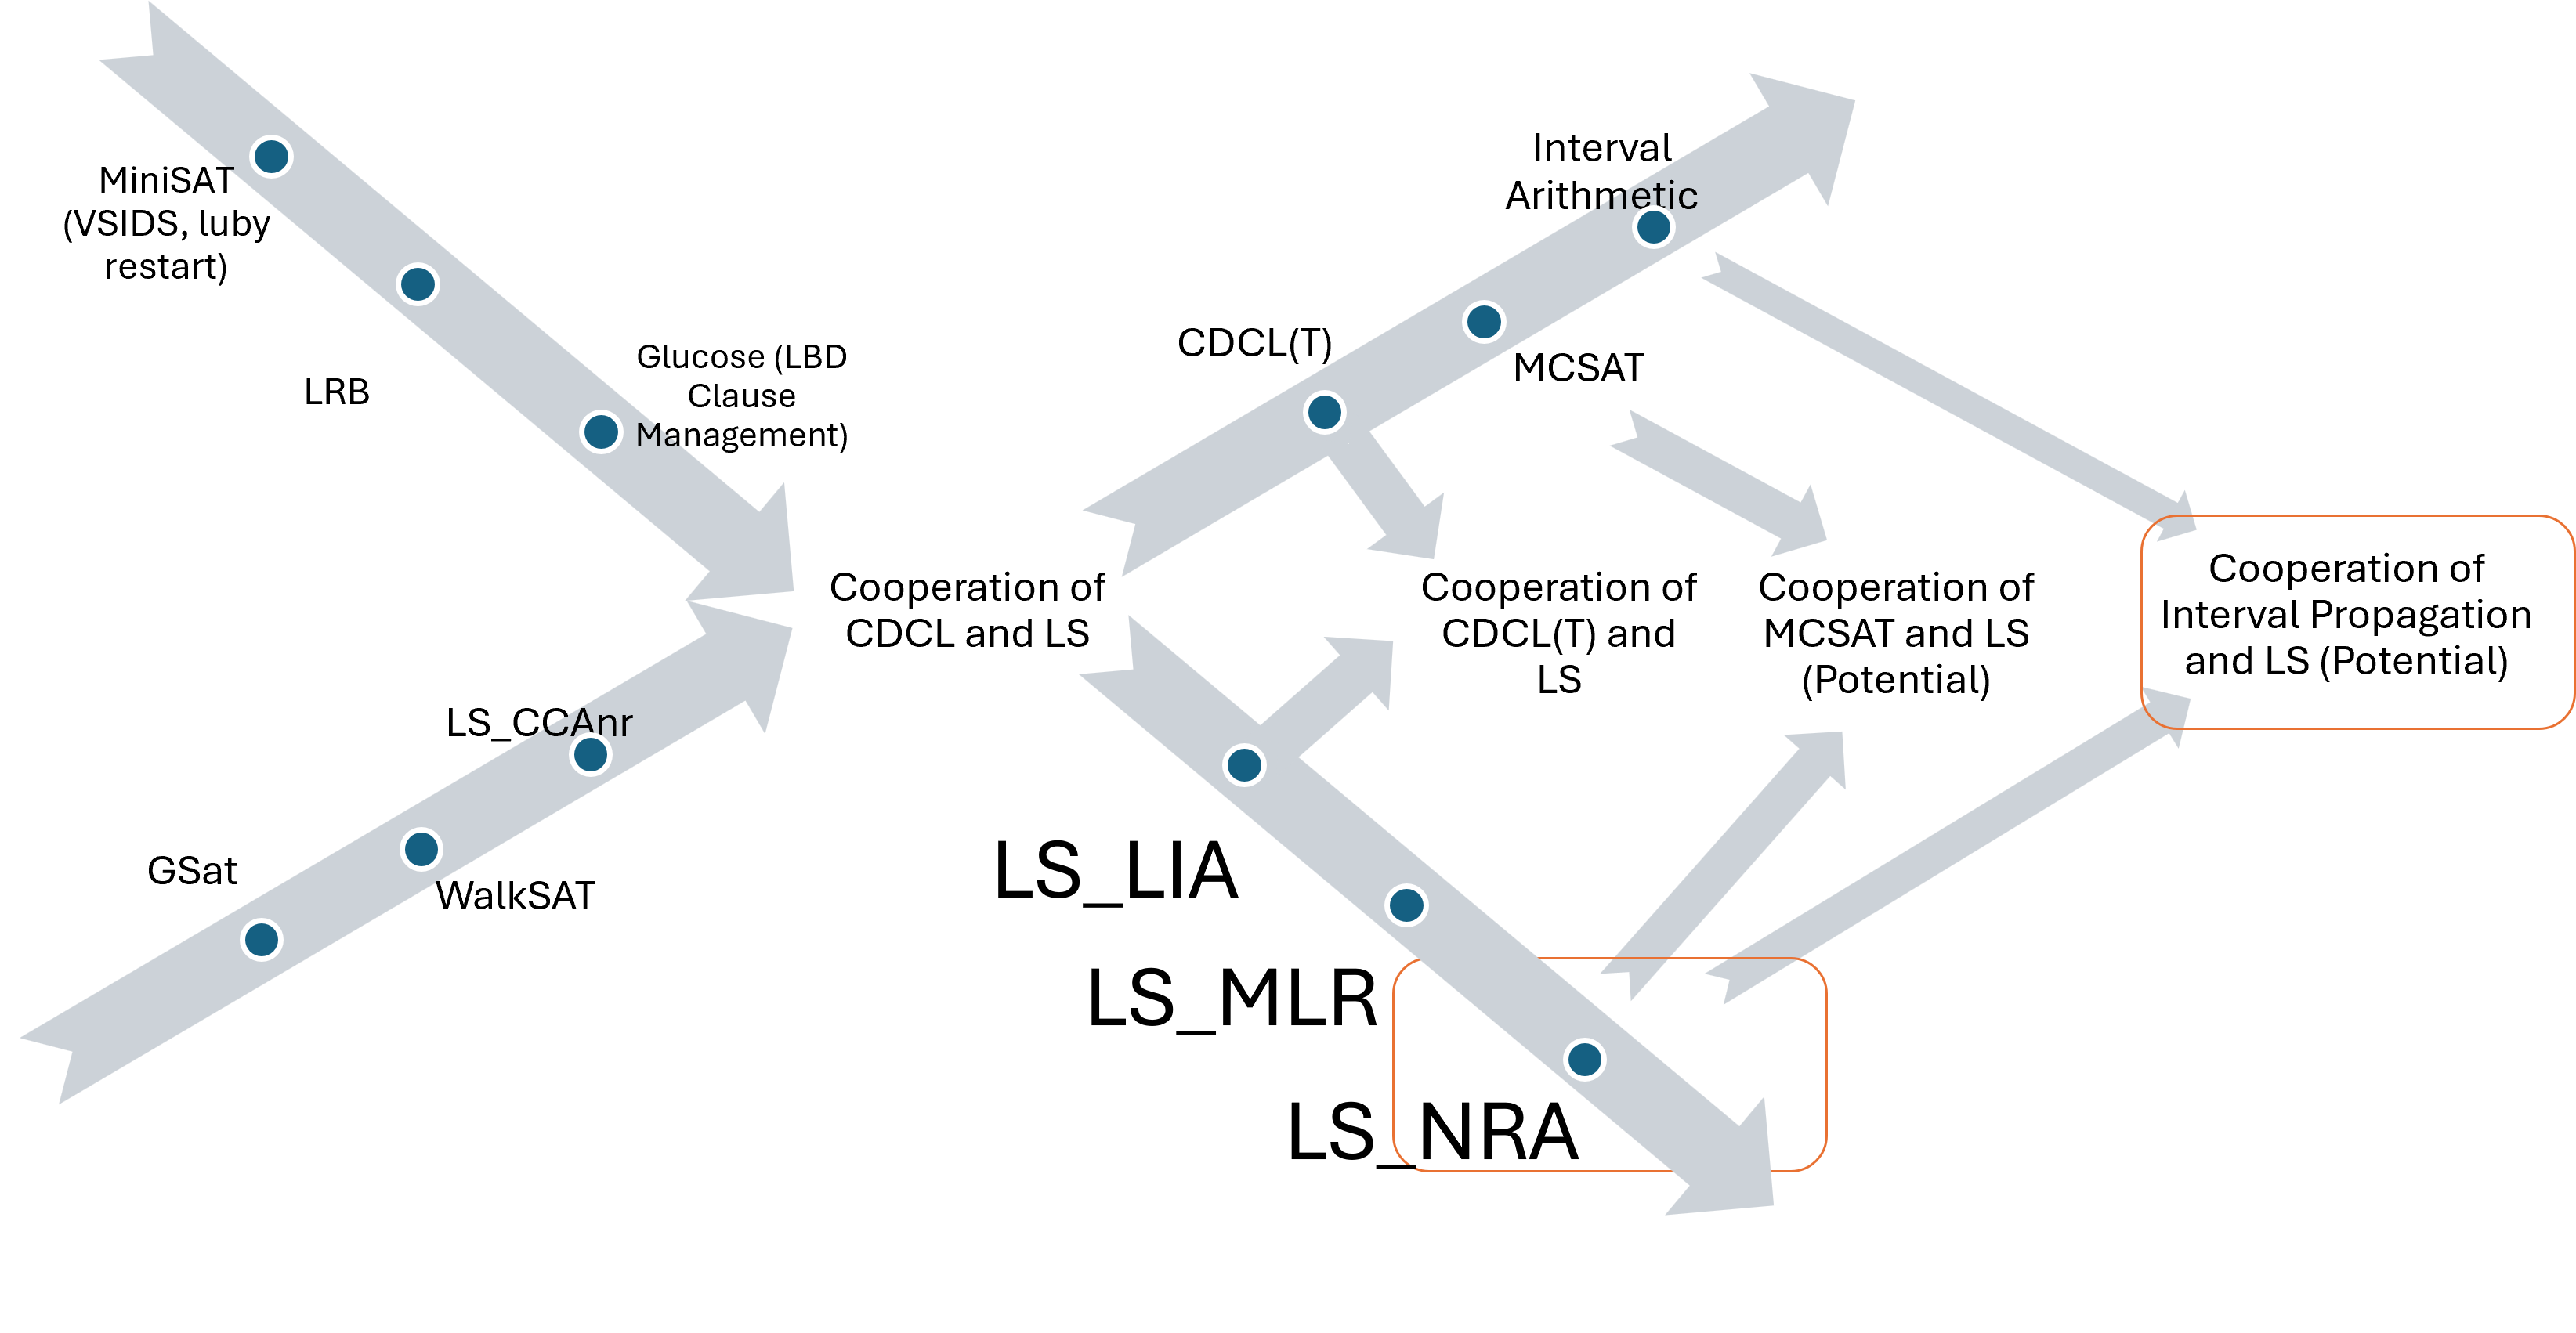
\includegraphics[width=\columnwidth]{Img/future.png}
%     \bicaption {局部搜索算法和完备算法的主要技术路线。} {Main Technical Routes of Local Search Algorithms and Complete Algorithms.}
% \label{fig:tech}
% \end{figure*}

\subsection{CDCL(T)算法}
CDCL(T) (Conflict Driven Clause Learning for Theories)算法主要是在SAT问题的CDCL搜索框架上增加了理论求解器(Theory Solver),主要的搜索思路包括单元传播、分支决策、冲突分析及回退等CDCL常见技术。理论求解器的作用是对给定的布尔骨架赋值进行推理,当全部布尔骨架得到赋值时通过理论分析返回问题可满足或者报告冲突。具体框架请参见图\ref{fig:cdclt}。

非线性实数的理论求解器主要目的是判断多项式不等式集合的一致性,主要方法可以分为以下几种:
\begin{itemize}
    \item \textbf{区间约束传播(interval constraint propagation, ICP):} 通过变量或者单项式的赋值区间推导出多项式的赋值区间,根据这些区间快速判断一些常见的不一致性。
    \item \textbf{虚拟替代(virtual substitution, VS):} 通过替换多项式中的变量,将多项式转化为更简单的形式,进而判断问题的可满足性。
    \item \textbf{柱形代数分解(cylindrical algebraic decomposition, CAD):} 如前文所述,通过把$R^n$空间划分为多个符号一致的胞腔,逐一排查的方式来推出问题的可满足性。
    \item \textbf{增量线性化(incremental linearization):}把一些多项式线性化,然后使用线性求解器检测问题可满足性,一般是不完备的。
\end{itemize}

\begin{figure*}[t]
    \centering
    \bicaption {CDCL(T)框架示意图} {Demo of CDCL(T) Framework.}
    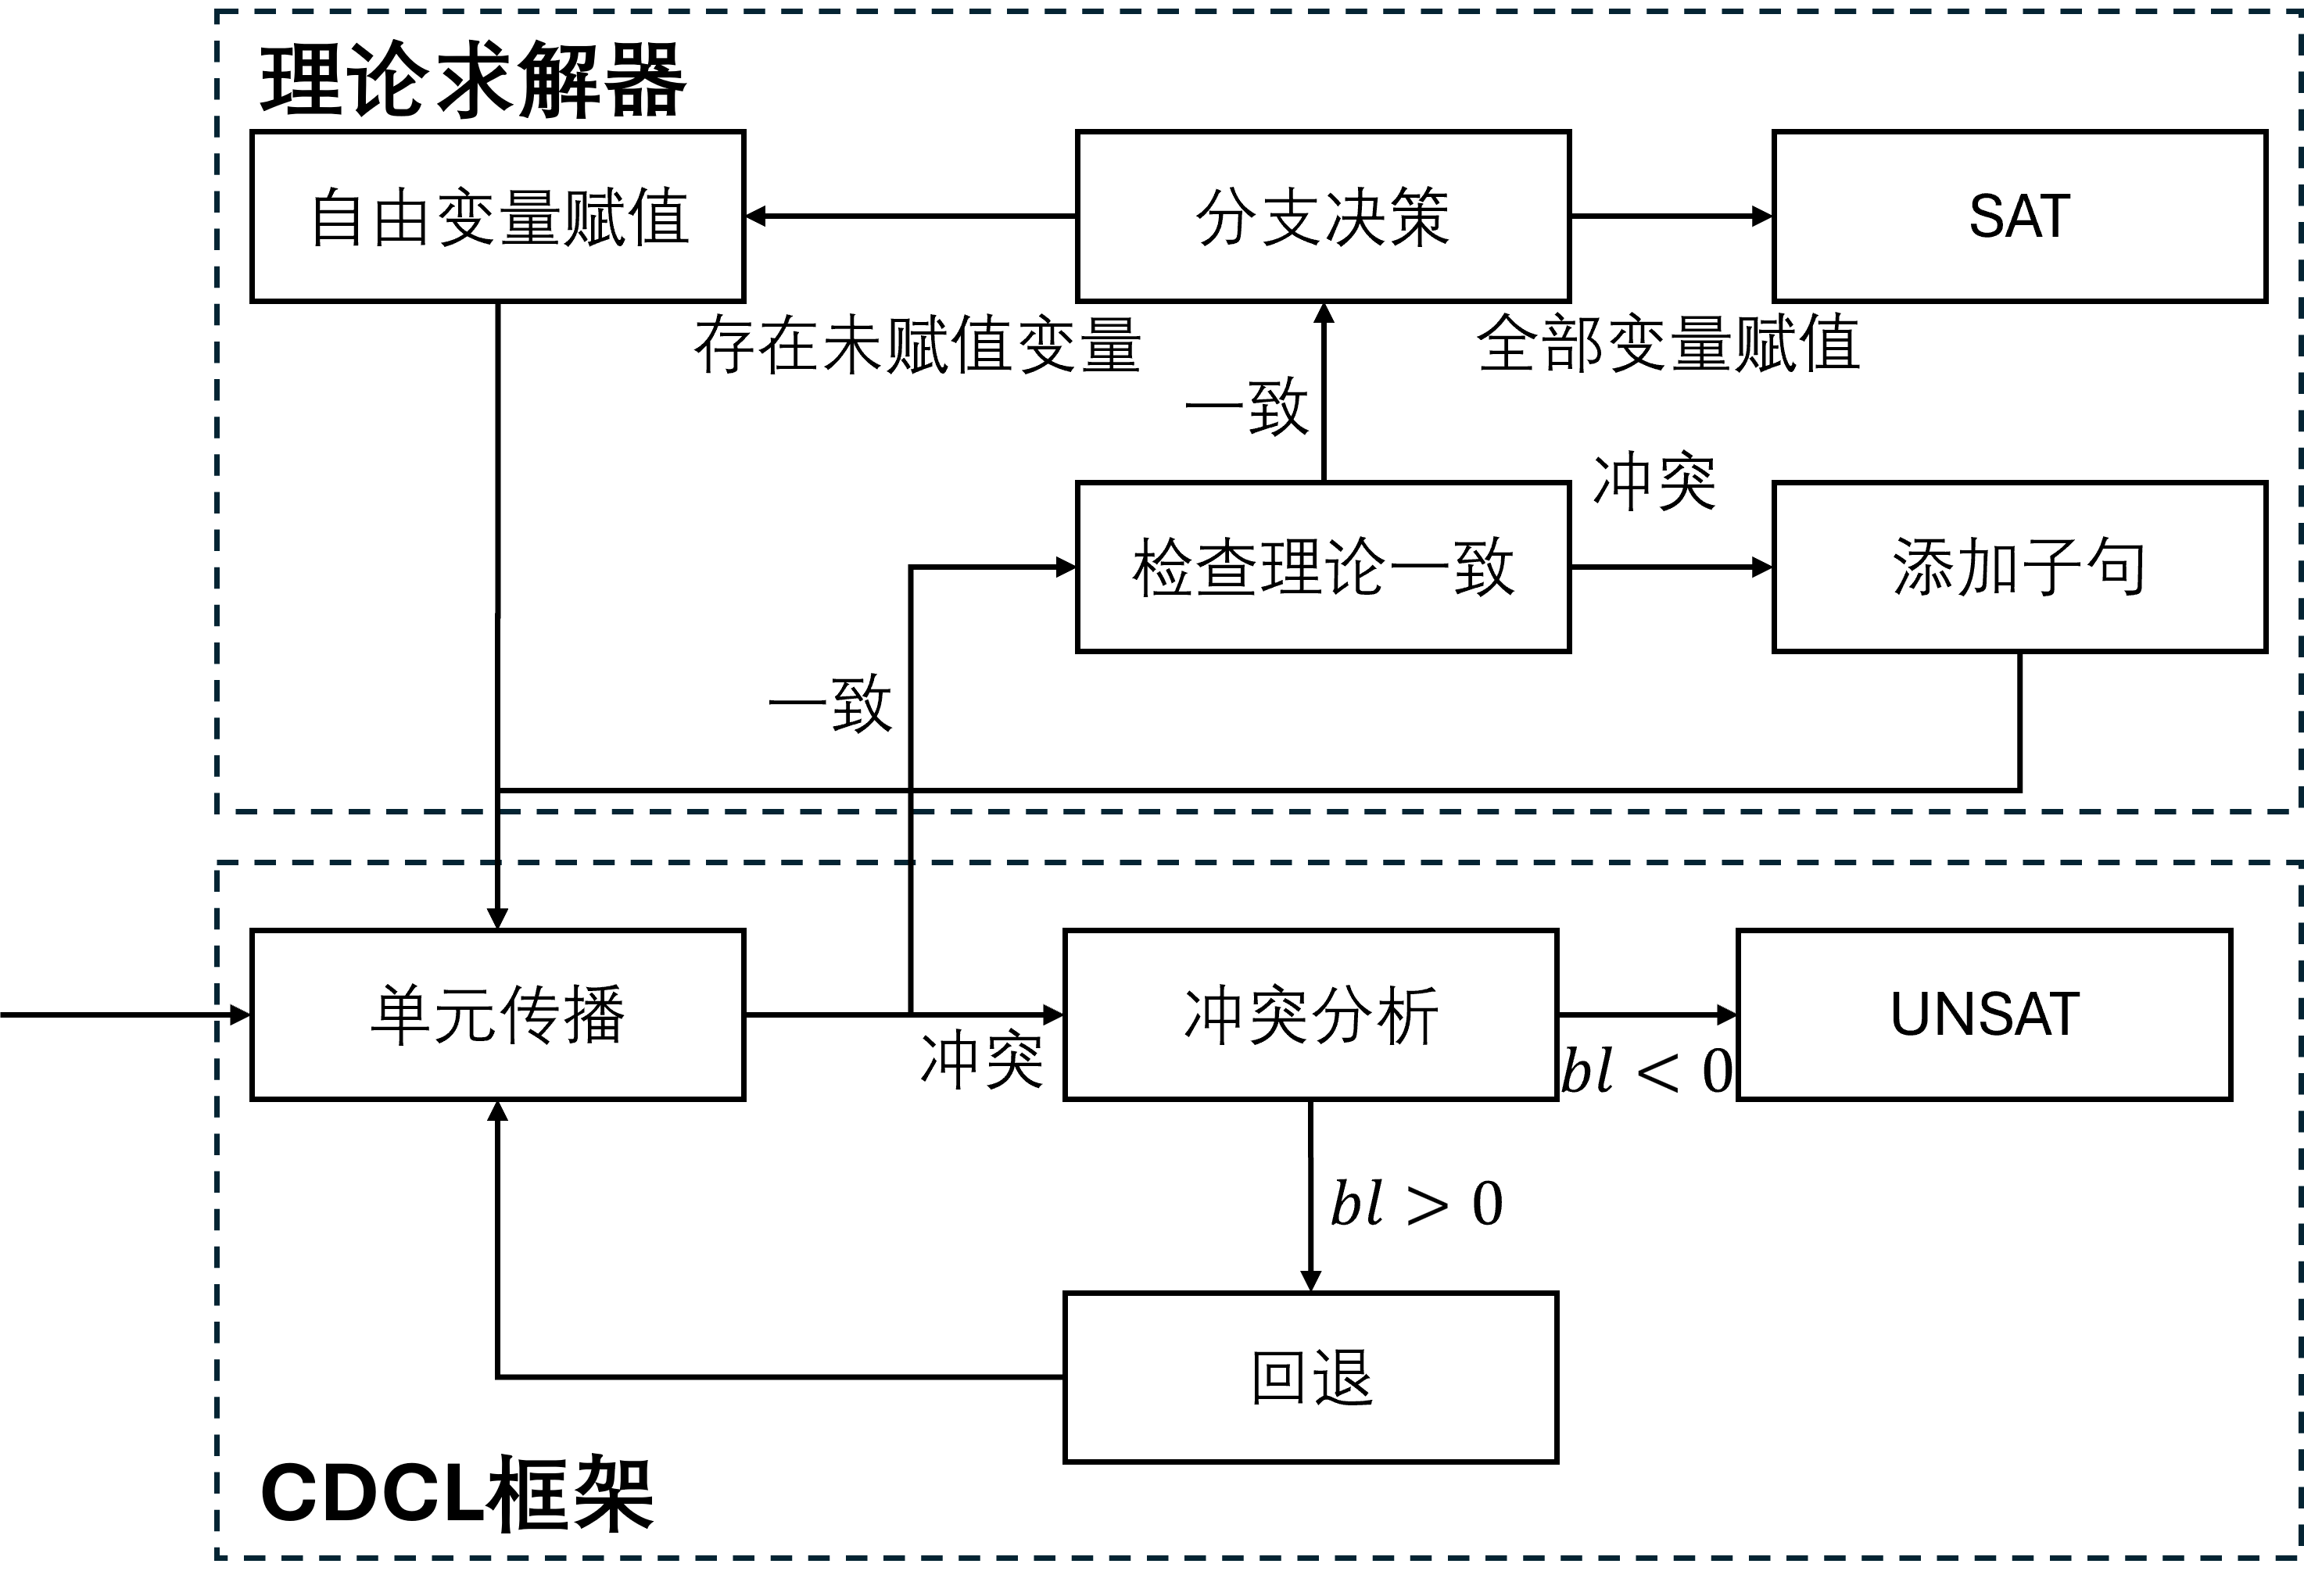
\includegraphics[width=0.6\columnwidth]{Img/cdcl_t.png}
    \label{fig:cdclt}
\end{figure*}

\subsection{MCSAT/NLSAT方法}
MCSAT(Model-Constructing Satisfiability)和NLSAT(NonLinear Satisfiability)是另外具有CDCL结构的算法,核心的思想仍然是决策赋值、冲突分析和回退。与CDCL(T)不同的是,MCSAT/NLSAT算法加入了基于可行域的算术变量推理,允许在脱离布尔骨架的情况下直接对算术变量进行赋值,一些基本概念介绍如下:
\begin{itemize}
    \item \textbf{决策层数(level):}指文字层面的决策层数,包括布尔文字和算术文字。
    \item \textbf{决策阶段(stage):}指算术变量赋值次数。
    \item \textbf{算法记录(trace):}一种记录算法更新的线性结构,包括可行域的更新、决策变量的赋值等。
    \item \textbf{算术传播(arithmetic propagation):}基于可行域的文字层面的传播,可以直接推断某些文字的可满足性。
\end{itemize}
其中,MCSAT/NLSAT最关键的步骤就是根据当前变量和文字的可行域关系进行算术文字赋值,假设算术变量的可行域是$curr\_set$,文字的可行域是$lit\_set$,算术区间传播分为以下几种情况:
\begin{itemize}
    \item \textbf{$lit\_set = \emptyset$:}任何赋值都不能使文字满足,判断文字为$\bot$。比如当$x \mapsto -1$时,文字$y^2 \leq x$不可满足。
    \item \textbf{$lit\_set = R$:}任何赋值都可以使文字满足,直接赋值文字为$\top$。比如文字$x^2 \geq -1$一定满足。
    \item \textbf{$curr\_set \subseteq lit\_set$:}当前文字的可行域包括了算术变量的可行域,因此可以直接判断文字满足。比如当$x \in [-2, 2]$时,文字$x^2 \leq 10$一定满足。
    \item \textbf{$curr\_set \cap lit\_set = \emptyset$:}任何可行域内的赋值都不会让文字满足,因此直接赋值文字为$\bot$。比如当$x \in [-2, 2]$时,文字$x^2 \geq 10$不可满足。
\end{itemize}

具体流程可参见图\ref{fig:mcsat}。搜索模块(Search)主要负责文字层面的单元传播和算术可行域层面的区间约束传播,当没有遇到冲突时,继续进行决策赋值;冲突可以由单元传播(子句中所有文字赋值为$\bot$)、算术区间传播(变量的可行域为空)产生。当发生冲突时,算法首先调用冲突分析,然后进入解释模块(Explain)。基于CAD的MCSAT算法原理是排除导致当前冲突赋值的胞腔,具体方法为首先调用CAD算法的投影和提升过程来得到冲突胞腔,然后学习对应胞腔的子句添加到搜索模块中。之后的搜索会在计算可行域时考虑新添加的子句,因此避免了重复陷入同一个冲突胞腔中。
例\ref{ex:nlsat}给出了一个MCSAT/NLSAT搜索的具体例子。

\begin{figure*}[t]
    \centering
    \bicaption {基于CAD的MCSAT框架示意图} {Demo of CAD-based MCSAT Framework.}
    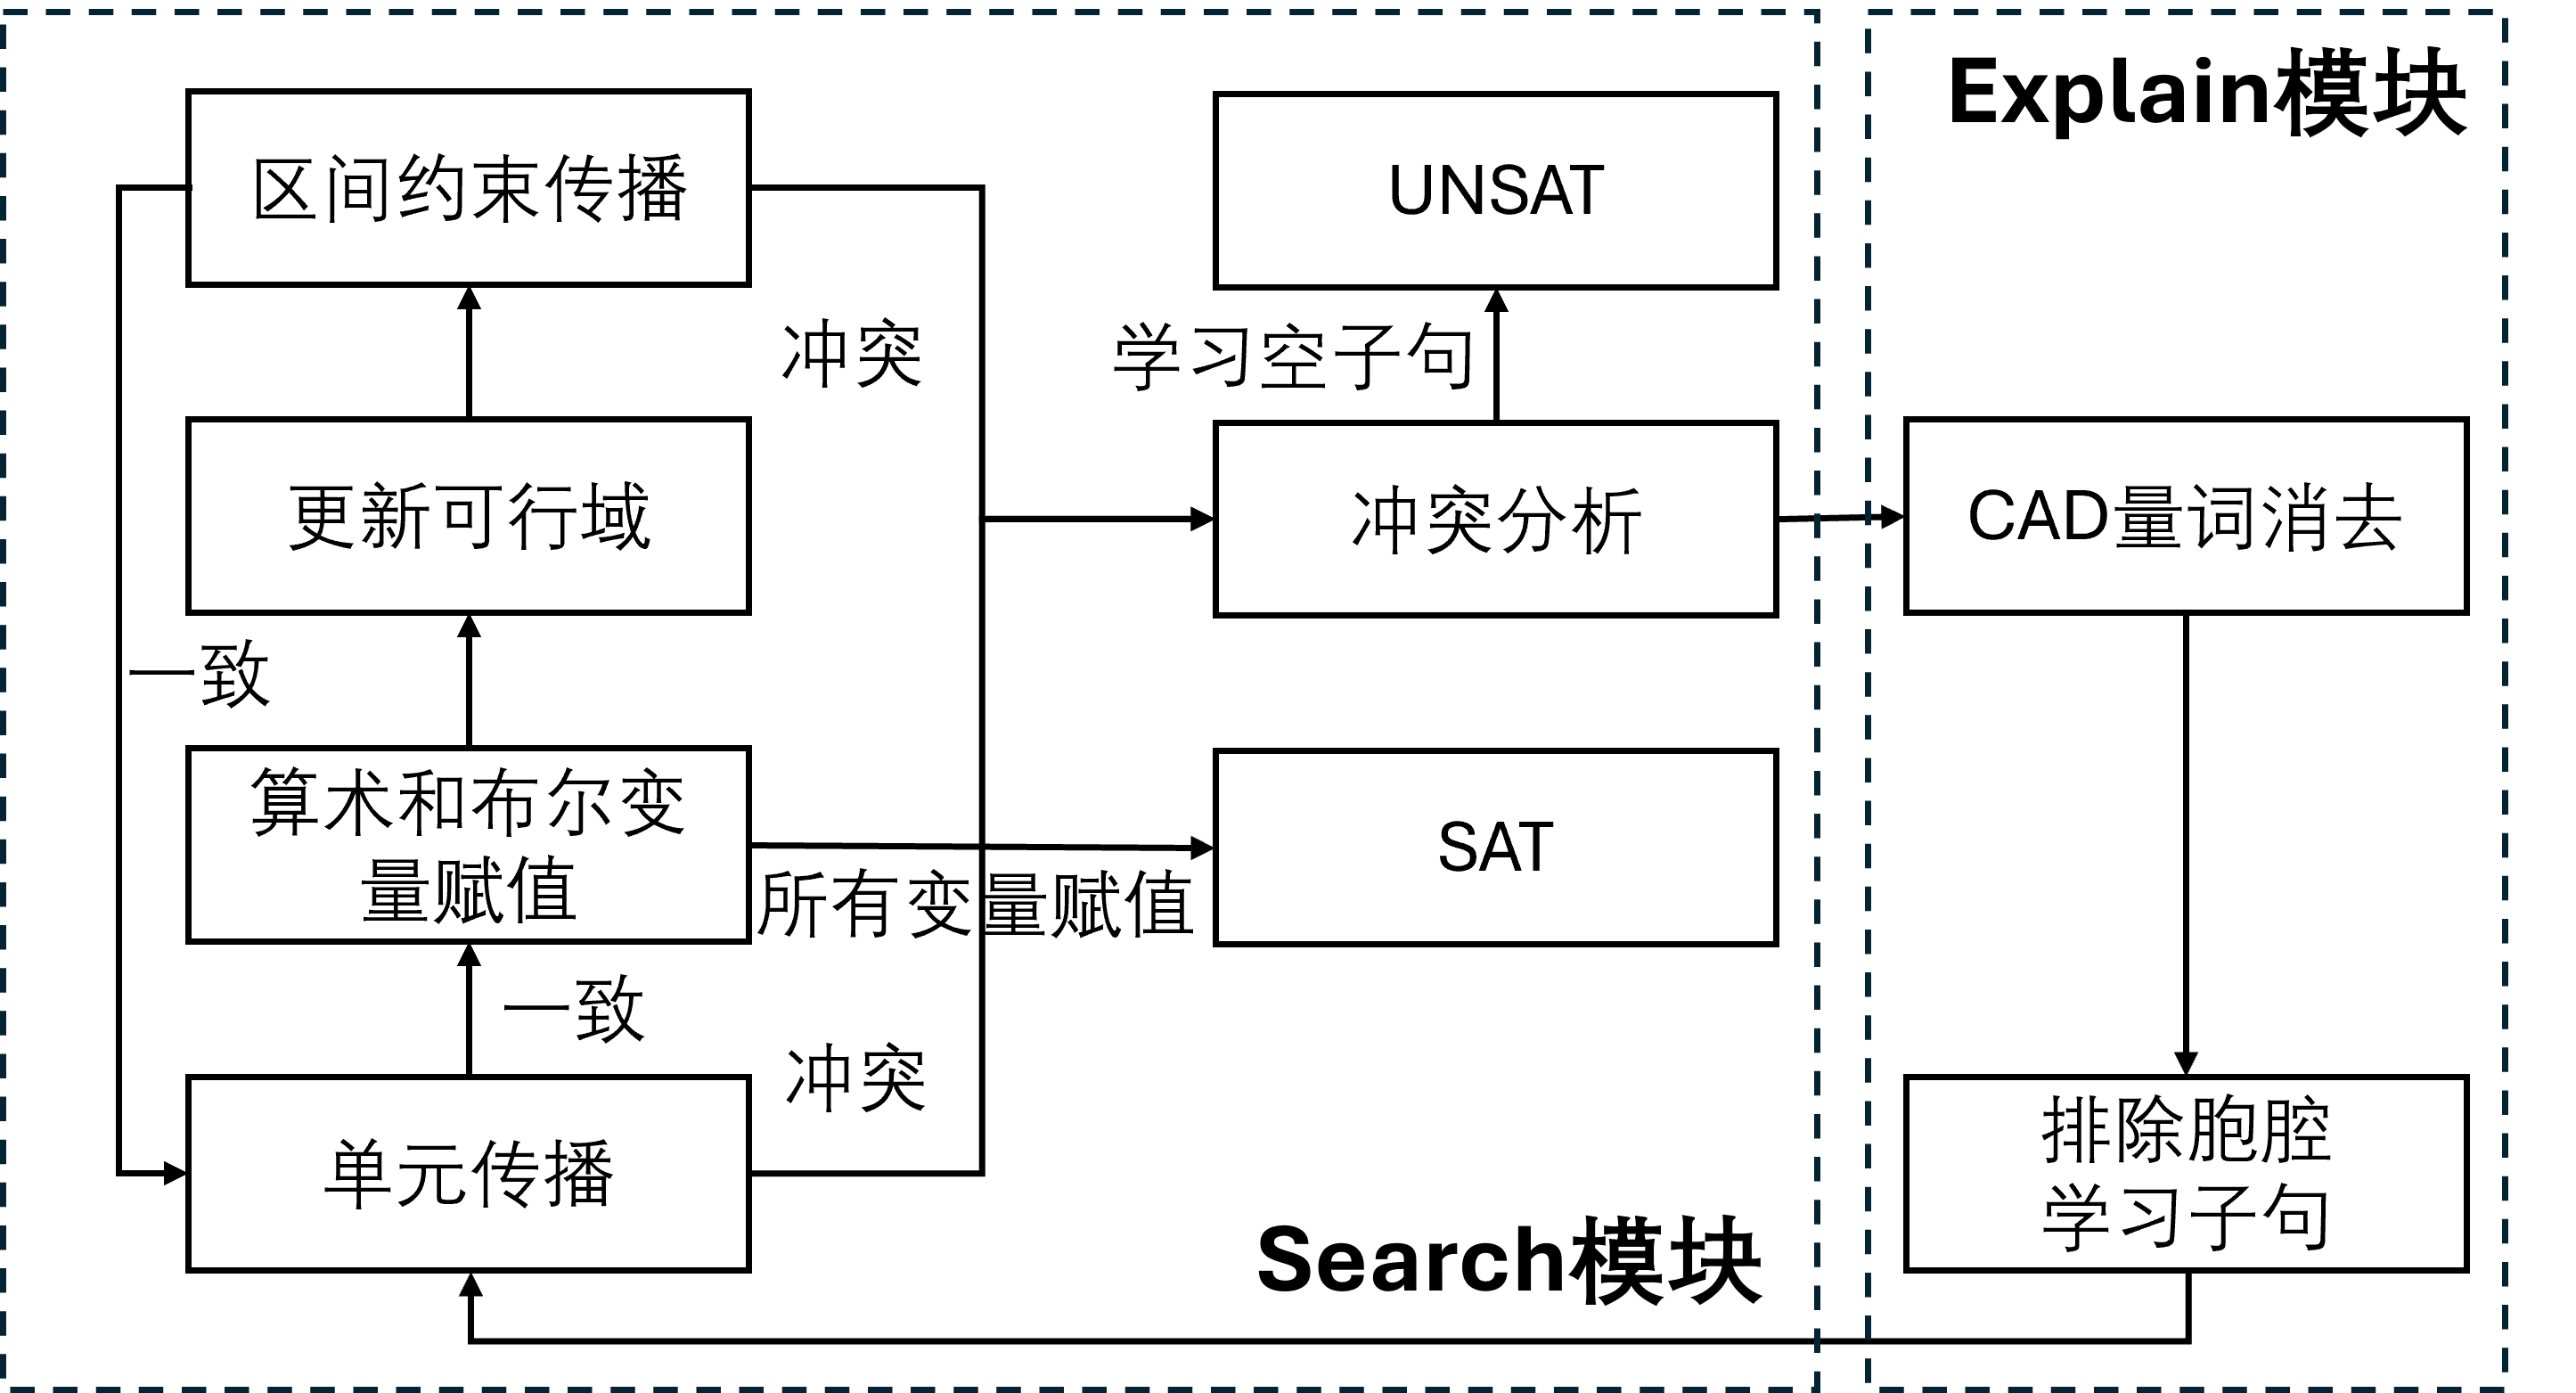
\includegraphics[width=0.6\columnwidth]{Img/mcsat.png}
    \label{fig:mcsat}
\end{figure*}


\begin{example}
考虑公式$F=(P_1: (x-2)^2 + y^2 \le 4) \wedge (P_2: x - y \ge 0)$。假设搜索顺序是$x < y$,算法的搜索过程如下:
\begin{enumerate}
    \item \textbf{决策算术变量:}赋值$x \mapsto 5$。
    \item \textbf{可行域计算:}计算$P_1$关于变量$y$的可行域是$\emptyset$,发现冲突。
    \item \textbf{冲突分析:}对公式$\exists y. (x-2)^2 + y^2 \le 4$进行量词消去,通过柱形代数分解得到实根$\{0, 4\}$,生成新的学习子句$x \le 4$。
    \item \textbf{回退:}回退到x未赋值的状态。
    \item \textbf{决策算术变量:}重新赋值$x \mapsto 2$。
    \item \textbf{可行域计算:}计算$P_1$关于变量$y$的可行域是$[-2, 2]$,$P_2$关于变量$y$的可行域是$(-\infty, 2]$,取交集得到可行域是$[-2, 2]$。
    \item \textbf{决策算术变量:}赋值$y \mapsto 0$。所有变量得到赋值,返回SAT。
\end{enumerate}
\label{ex:nlsat}
\end{example}

\subsection{局部搜索算法现状}
局部搜索算法是一种启发式的非完备算法,它的主要思想是把SMT问题看作是一个优化问题,通过迭代操作找到最终的可行解。一般来说,局部搜索只能用来求解可满足问题,而不能证明问题的不可满足性。首先给出基本概念的定义如下:

\begin{definition}{\textbf{状态 (State)}}
状态是指问题的一个解,比如变量的一组赋值。
\end{definition}

\begin{definition}{\textbf{操作 (Operation)}}
操作是每一次迭代需要做的状态上的改变,SMT问题的状态是修改变量的赋值。假设移动前后的状态为$S$和$S'$,操作是$op$,记为$S \xrightarrow{op} S'$。
\end{definition}

\begin{definition}{\textbf{打分函数 (Scoring Function)}}
打分函数是一个状态到实数的函数,用来评估状态的好坏。一般认为离目标越远的状态分数越低。操作的打分函数被定义为状态改变前后分数的差值。
\end{definition}

\begin{definition}{\textbf{邻域 (Neighbourhood)}}
邻域表示的是状态空间的邻居。假设当前状态为$S$,邻域是指所有通过一次操作$op$可以到达的状态的集合,即$N(S) = \{S' : S \xrightarrow{op} S'\}$。
\end{definition}

假设状态空间$S$为所有候选解构成的解空间,局部搜索的具体求解过程可以概括如下:
\begin{enumerate}
    \item 随机生成一个初始状态$s_0 \in S$。一般来说,初始状态可以启发式生成,尽量减小约束的复杂度。
    \item 定义操作$op$,同时定义邻域函数$N: S \rightarrow 2^S$,表示从状态$S$可以到达的状态集合。这样,找到了从初始状态可以到达的一系列候选状态$N(s_0)$
    \item 定义打分函数$f: S \rightarrow R$,表示状态的好坏。贪心地从候选状态中找到分数最好的一个进行迭代。
    \item 设置停止条件,比如最大迭代次数、最大限制时间,或者已经找到问题的最优解。
    \item 迭代搜索2-3步,直到满足停止条件4。
\end{enumerate}
对于SMT问题而言,工作\cite{CaiLZ2023}给出了一种实例化的概念:
\begin{itemize}
    \item 初始解:一般通过变量的上下界来选取,比如当变量$v$的上下界为$[-2, 3]$时,可以选择初始状态为$v \mapsto 0$。
    \item 单变量关键操作:SMT问题的操作定义为让一个约束满足的赋值变量进行变化。比如对于约束$x + y \geq 2$,当前状态为$\{x \mapsto 1, y \mapsto 0\}$,则有以下两种操作:
    \begin{itemize}
        \item 保持变量$x$不变,增加变量$y$的值,使约束满足,比如$y \mapsto 1$。
        \item 保持变量$y$不变,增加变量$x$的值,使约束满足,比如$x \mapsto 2$。
    \end{itemize}

    \item 邻域:邻域是所有通过一次操作可以到达的状态的集合$\{S' : S \xrightarrow{op} S'\}$,单变量关键操作的邻域是只有一个变量不同的状态集合,即$N(S) = \{N(S): \exists v \in V: S(v) \neq S'(v) \land \forall v' \in V / \{v\}: S(v) = S'(v) \}$。
\end{itemize}

工作\cite{CaiLZ2023}为求解算术理论的局部搜索算法给出了一个基本的框架,如算法\ref{alg:basic}所示。

\begin{algorithm}[t]
    % \small
    \caption{Basic local search algorithm}
    \label{alg:basic}
    \textbf{输入}: A set of clauses $F$\\
    \textbf{输出}: An assignment that satisfy $F$, or failure\\
    
    \begin{algorithmic}[1] %[1] enables line numbers
        \Statex \hrulefill
        \STATE Initialize assignment randomly;
        \While{\top}
            \IF{all clauses are satisfied}
                \RETURN current assignment;
            \ENDIF
            \IF{time or step limit reached}
                \RETURN failure;
            \ENDIF
            \STATE $var, new\_val, score \leftarrow best critical move$;
            \IF{$score > 0$}
                Perform move, assign $v \mapsto new\_val$;
            \ELSE
                \STATE Update clause weight according to PAWS scheme;
                \STATE $cls \leftarrow random unsatisfied clause$;
                \STATE $var, new\_val, score \leftarrow best move(cls)$;
                \IF{$score \neq -\infty$}
                    Perform move, assign $v \mapsto new\_val$;
                \ENDIF
                \IF{no move performed previously}
                \STATE Randomly change assignment of some variables;
                \ENDIF
            \ENDIF
        \EndWhile
    \end{algorithmic}
\end{algorithm}

下面以一个具体的例子\ref{ex:ls}进行说明。
\begin{example}
    假设当前SMT约束$F = \{C_1: x + y \leq 2, C_2: 2x + 3y \geq 5\}$,=目标是找到一个满足约束的解。通过局部搜索算法进行求解的具体步骤如下:

    \begin{enumerate}
        \item \textbf{初始解生成:} 初始赋值$\{x \mapsto 0, y \mapsto 0\}$。当前赋值满足约束$C_1$,但不满足约束$C_2$。
        \item \textbf{生成操作:} 考虑未满足约束$C_2$,可以固定变量$x$或$y$的赋值,比如赋值$op_1: \{x \mapsto 0, y \mapsto 2\}$,或者$op_2: \{x \mapsto 3, y \mapsto 0\}$。
        \item \textbf{打分函数:} 打分函数设计为移动前后约束权重的差值,操作$op_1$可以满足两种约束,而操作$op_2$在满足约束$C_2$的同时破坏了约束$C_1$。
        \item \textbf{移动操作:} 选择操作$op_1$,移动后赋值为$\{x \mapsto 0, y \mapsto 2\}$。
        \item \textbf{算法停止:} 当所有约束都满足时,算法停止,返回当前赋值。
    \end{enumerate}
\label{ex:ls}
\end{example}

\subsection{混合求解方法}
近年来,混合求解方法\cite{CaiZ21}成为求解SAT和SMT方法的高效方法之一,其主要思想是结合完备算法的推理能力和局部搜索算法的采样能力。对于一个约束公式,混合求解方法首先使用完备算法进行单元传播,然后在目标可行解附近时(依赖于启发式判断)无视冲突进行赋值的拓展,然后调用局部搜索算法在邻域迭代,企图可以解决当前的冲突。除此之外,混合求解算法为两种求解模式的求解信息提供了桥梁,比如使用变量的冲突频率来加速完备算法的分支决策和相位选择等。

对于SMT问题而言,目前的混合求解方法\cite{hybridSMT}将其抽象为布尔骨架,然后对相应的文字做SAT混合求解方法一样的处理,即使用算术局部搜索方法加速CDCL(T)算法的求解过程。工作\cite{BoostMcsat}则在MCSAT框架上与局部搜索算法做深度耦合,MCSAT为局部搜索算法提供完整的初始赋值,而局部搜索算法则用来为MCSAT算术变量决策提供指导。

\section{本章小结}

本章节主要介绍了SMT非线性算术问题的相关概念和研究现状。
首先,本文给出逻辑公式的形式化定义,包括文字、子句、赋值等基本概念,然后引出非线性多项式及对应的可满足问题。
然后,本文讨论了SMT问题的解空间,并讨论了柱形代数分解求得解空间胞腔的方法。
最后,本文介绍了目前的几种求解方法,包括CDCL(T)、MCSAT和局部搜索算法。这些算法在实际应用中有着不同的优势和劣势,可以根据具体问题的特点选择合适的算法进行求解。